% Created 2024-10-09

% Title: scipy.cpp - Using AI to Port Python's scipy.signal Filter-Related Functions to C++ for Use in Real Time

% Edit Abstract: https://

% Abstract:

\begin{slide}[\slideopts,toc={NSMT}]{Neural Spectral Modeling Template (NSMT) --- Audio Image Classification}

% ADCxGather2025 abstract 2025-08-24

%  \vspace{-1.5em}
  
% Final onboarding: https://conference.audio.dev/wp-admin/post.php?post=25949&action=edit&var=registration

  \begin{itemize}

    \mpitem Adapts state-of-the-art image-classification tools to spectral audio modeling

    \mpitem Started as a fork of the \emph{Lightning Hydra Template (LHT):} \url{https://github.com/ashleve/lightning-hydra-template}
    \begin{itemize}

      \mpitem PyTorch Lightning streamlines deep-learning model development in
      numerous ways

      \mpitem Hydra is a powerful configuration management framework often used

      \mpitem An LHT \emph{example experiment} trains an MLP on MNIST (hand-written digits)

    \end{itemize}

    \mpitem NSMT adds \emph{more architectures:} CNNs, ConvNeXt, EfficientNet, ViT

    \mpitem NSMT adds \emph{more datasets:} CIFAR-10, CIFAR-100, VIMH

    \mpitem Variable Image Multi-Head (VIMH) format generalizes CIFAR-100:
    \begin{itemize}
      \mpitem Up to 65k x 65k images with up to 65k channels (``stacked spectral representations'')
      \mpitem \emph{Multi-Head support:} \emph{separate classification/regression head per category}
      \mpitem \emph{Data loaders} for the various datasets and model architectures
      \mpitem The \texttt{configs/experiment/} directory contains \emph{benchmark replications} % on MNIST, CIFAR, and VIMH datasets
      \mpitem Top-level \texttt{Makefile} contains $\approx100$ \emph{make targets} for tests, training, experiments
    \end{itemize}
  \end{itemize}

\end{slide}

\begin{slide}[\slideopts,toc={Spectra}]{Why Spectral Representations}

  Aren't we supposed to be doing everything \emph{end to end} now?

  Shouldn't the input be a digital audio \emph{bit stream} by now?

  \begin{itemize}

    \mpitem Sure, you can do it that way, but with \emph{far more}
    \begin{itemize}
      \mpitem training \emph{data},
      \mpitem training \emph{time}, 
      \mpitem computational complexity (e.g., Transformer)
    \end{itemize}
    \mpitem It is more cost-effective to exploit \emph{inductive priors:}
    \begin{itemize}
      \mpitem The \emph{ear} is a \emph{hardware spectrum analyzer} used for all audio perception
      \mpitem \emph{Superhuman hearing} is possible using a \emph{stack of different time-frequency resolutions}\\
      (Multi-Scale Spectrograms)
      \mpitem Any additional feature can be brought in as a \emph{conditioning} input\\
      (such as \emph{pre-emphasis})
    \end{itemize}

  \end{itemize}

  \vspace{-1em}
%  \begin{quote}
\maybepause
    \centerline{\textit{Those who don't know signal processing are doomed to reinvent it}}
\maybepause
    \centerline{\textit{Those who know signal processing are doomed to re-introduce it}}
%  \end{quote}

\end{slide}

\begin{slidewhite}[\slideopts,toc={Problem}]{Example Driving Problem: Real-Time Filter Design in an Audio Plugin}

  \vspace{-2em}
  \myFigureRotateToWidth{pgmeejos}{-90}{0.85\twidth}{(Red-Bordered Buttons Added to
    \textbf{Plugin GUI Magic}'s Equalizer Example)}

\end{slidewhite}

\begin{slide}[\slideopts,toc={CNN}]{SimpleCNN Architecture}
  
  \emph{Convolutional Neural Network for Spatial Feature Extraction}
  
  \begin{itemize}
    \mpitem \emph{Two conv layers:} 3×3 kernels, 32→64 channels, MaxPool, BatchNorm
    
    \mpitem \emph{Adaptive pooling:} 7×7 feature maps → FC classifier with dropout
    
    \mpitem \emph{Parameter variants:} 8K (small), 68K (medium), 421K (large)
    
    \mpitem \emph{Performance:} CIFAR-10: 85-92\%, CIFAR-100: 55-70\%
    
    \mpitem Supports multihead classification for multi-task learning
  \end{itemize}
  
  \vspace{0.5em}
  \centerline{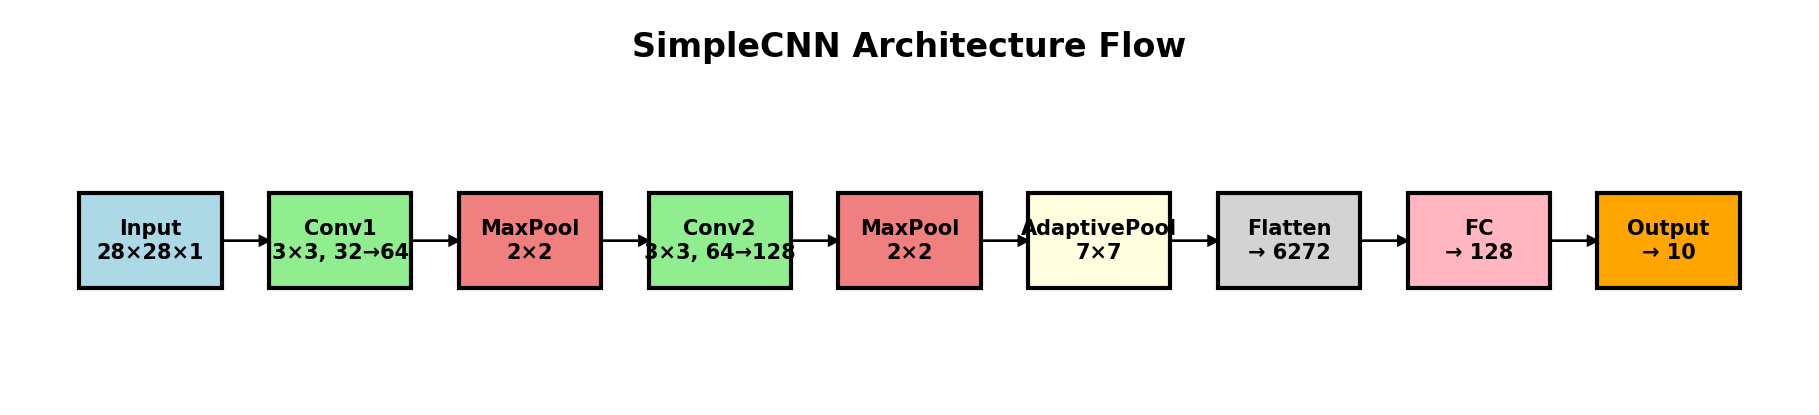
\includegraphics[width=0.9\textwidth]{viz/diagrams/cnn_architecture.eps}}
\end{slide}

\begin{slide}[\slideopts,toc={ConvNeXt}]{ConvNeXt-V2 Architecture}
  
  \emph{Modern CNN with Global Response Normalization (GRN)}
  
  \begin{itemize}
    \mpitem \emph{Key innovation:} GRN normalizes across spatial/channel dimensions
    
    \mpitem \emph{Architecture:} 7×7 depthwise conv, LayerNorm, 4× MLP with GELU
    
    \mpitem \emph{Sizes:} Tiny (18K), Small (73K), Base (288K), Large (725K)
    
    \mpitem \emph{Best performer:} CIFAR-10: 90-95\%, CIFAR-100: 70-80\%
  \end{itemize}
  
  \vspace{0.5em}
  \centerline{\includegraphics[width=0.9\textwidth]{viz/diagrams/convnext_architecture.eps}}
\end{slide}

\begin{slide}[\slideopts,toc={EfficientNet}]{EfficientNet Architecture}
  
  \emph{Optimized CNN for Mobile and Edge Deployment}
  
  \begin{itemize}
    \mpitem \emph{Compound scaling:} Balances depth, width, and resolution
    
    \mpitem \emph{Mobile-optimized:} Inverted residuals, squeeze-excitation, Swish
    
    \mpitem \emph{Sizes:} 22K (edge), 210K (balanced), 7M (high accuracy)
    
    \mpitem \emph{Performance:} CIFAR-10: 89-94\%, CIFAR-100: 67-77\%
  \end{itemize}
  
  \vspace{0.5em}
  \centerline{\includegraphics[width=0.9\textwidth]{viz/diagrams/efficientnet_architecture.eps}}
\end{slide}

\begin{slide}[\slideopts,toc={ViT}]{Vision Transformer (ViT) Architecture}
  
  \emph{Attention-Based Learning on Image Patches}
  
  \begin{itemize}
    \mpitem \emph{Image → Patches:} 28×28 → 7×7 patches → token sequence
    
    \mpitem \emph{Self-attention:} Multi-head attention + MLP with GELU
    
    \mpitem \emph{Sizes:} Tiny (38K), Small (210K, MNIST SOTA: 99.5\%), Base (821K)
    
    \mpitem Highly parallelizable, scales with data and compute
  \end{itemize}
  
  \vspace{0.5em}
  \centerline{\includegraphics[width=0.9\textwidth]{viz/diagrams/vit_architecture.eps}}
\end{slide}

\begin{slide}[\slideopts,toc={CIFAR-10}]{CIFAR-10 Dataset Support}
  
  \emph{Standard Computer Vision Benchmark}
  
  \begin{itemize}
    \mpitem 10 classes, 32×32 RGB, 50K train / 10K test
    
    \mpitem \emph{NSMT Results:} CNN (85-92\%), ConvNeXt (90-95\%), ViT (88-93\%)
    
    \mpitem \emph{Commands:} \texttt{make cbq10c} (quick), \texttt{make cb10c} (full)
    
    \mpitem Literature-competitive performance out-of-the-box
  \end{itemize}
  
  \vspace{0.5em}
  \centerline{\includegraphics[width=0.9\textwidth]{viz/diagrams/cifar10_samples.eps}}
\end{slide}

\begin{slide}[\slideopts,toc={CIFAR-100}]{CIFAR-100 Dataset Support}
  
  \emph{Fine-Grained Classification Challenge}
  
  \begin{itemize}
    \mpitem 100 fine classes or 20 coarse superclasses, 32×32 RGB
    
    \mpitem \emph{Performance:} ConvNeXt leads at 70-80\% (fine), 85\% (coarse)
    
    \mpitem \emph{Multihead:} Simultaneous fine + coarse classification
    
    \mpitem \emph{Commands:} \texttt{make cb100c}, \texttt{make cbs100}
  \end{itemize}
  
  \vspace{0.5em}
  \centerline{\includegraphics[width=0.9\textwidth]{viz/diagrams/cifar100_samples.eps}}
\end{slide}

\begin{slide}[\slideopts,toc={VIMH}]{Variable Image MultiHead (VIMH) Format}
  
  \emph{Generalized Dataset Format for Multi-Parameter Learning}
  
  \begin{itemize}
    \mpitem \emph{Self-describing:} Variable dimensions up to 65k×65k×65k (16-bit metadata)
    
    \mpitem \emph{Flexible labels:} 0-255 parameters, 8-bit quantized (~100 steps)
    
    \mpitem \emph{Per sample:} [height, width, channels] + [N params] + [ID,val pairs] + image
    
    \mpitem \emph{Applications:} Audio spectrograms, vision, scientific data
    
    \mpitem Models auto-configure from dataset metadata
  \end{itemize}
  
  \vspace{0.5em}
  \centerline{\includegraphics[width=0.8\textwidth]{png/sample_data.eps}}
\end{slide}

\begin{slide}[\slideopts,toc={MultiHead}]{Multi-Head Classification Support}
  
  \emph{Training Networks with Multiple Output Tasks}
  
  \begin{itemize}
    \mpitem \emph{Architecture:} Shared backbone → separate heads per task
    
    \mpitem \emph{Task types:} Classification, ordinal regression, pure regression
    
    \mpitem \emph{Examples:} MNIST (digit+thickness), CIFAR-100 (fine+coarse)
    
    \mpitem Configurable via Hydra without code changes
  \end{itemize}
  
  \vspace{0.5em}
  \centerline{\includegraphics[width=0.8\textwidth]{viz/diagrams/multihead_architecture.eps}}
\end{slide}

\begin{slide}[\slideopts,toc={Benchmarks}]{Benchmark Replications \& Experiments}
  
  \emph{50+ Pre-Configured Experiments}
  
  \begin{itemize}
    \mpitem \emph{Categories:} MNIST, CIFAR-10/100, VIMH, Multihead
    
    \mpitem \emph{Features:} Fixed seeds, fair comparisons, automated tracking
    
    \mpitem \emph{Commands:} \texttt{make ca} (compare), \texttt{make cbqa} (quick), \texttt{make cbsa} (full)
    
    \mpitem Version-controlled configs ensure reproducibility
  \end{itemize}
\end{slide}

\begin{slide}[\slideopts,toc={Makefile}]{100+ Makefile Targets}
  
  \emph{Streamlined Research Workflow}
  
  \begin{itemize}
    \mpitem \emph{Abbreviations:} \texttt{t*} (train), \texttt{tq*} (quick), \texttt{cb*} (CIFAR), \texttt{e*} (experiments)
    
    \mpitem \emph{Progressive testing:} \texttt{tq} → \texttt{ca} → \texttt{cbqa} → \texttt{cbs}
    
    \mpitem \emph{Productivity:} \texttt{make help}, logical naming, batch operations
  \end{itemize}
\end{slide}

%% Example showing how figures can be brought in:
%% \begin{slidewhite}[\slideopts,toc={Problem}]{Example Driving Problem: Real-Time Filter Design in an Audio Plugin}
%%   \vspace{-2em}
%%   \myFigureRotateToWidth{pgmeejos}{-90}{0.85\twidth}{(Red-Bordered Buttons Added to
%%     \textbf{Plugin GUI Magic}'s Equalizer Example)}
%% \end{slidewhite}

\begin{slide}[\slideopts,toc={}]{Summary of Resources Online}
  \begin{itemize}
    \item \emph{Neural Spectral Modeling Template (NSMT):}\\
      \href{https://github.com/josmithiii/neural-spectral-modeling-template.git}
           {\texttt{github.com/josmithiii/neural-spectral-modeling-template}}
    \item[]
    \item \emph{Lightning Hydra Template Extended (LHTE):}\\
      \href{https://github.com/josmithiii/lightning-hydra-template-extended.git}
           {\texttt{github.com/josmithiii/lightning-hydra-template-extended}}
    \item[]
    \item \emph{Lightning Hydra Template (LHT):}\\
      \href{https://github.com/ashleve/lightning-hydra-template}
           {\texttt{github.com/ashleve/lightning-hydra-template}}
    \item[]
    \item JOS Home Page (Videos, Overheads, including these):\\
      \href{https://ccrma.stanford.edu/~jos/Welcome.html}
           {\texttt{https://ccrma.stanford.edu/\~{}jos/}}
  \end{itemize}
\end{slide}
